\chapter{التطبيق خطوة بخطوة}
\label{ch:walkthrough}

\section{ابدأ من القصة: ما الذي سننجزه؟}
\label{sec:start}

لنفترض أن لدينا مؤسسة اسمها «وزارة الاقتصاد والصناعة». تتبع لها «الإدارة العامة للتجارة الداخلية وحماية المستهلك»، وتحتها «مديرية حماية المستهلك وسلامة الغذاء»، ثم «دائرة حماية المستهلك». يعمل أحمد ونور وريم في هذه الدائرة. يريد الفريق تنظيم مراسلاته حول «فرن الأمانة»، بحيث يعرف كل شخص ما المطلوب منه، وتبقى الكتب والردود والقرارات في مكان واحد.

سنبدأ بكتاب داخلي بسيط: يكتب نور طلب تحديد موعد كشف على الفرن، تراجعه ريم، ويوقّعه أحمد. ثم نعالج كتاباً وارداً من الفرن، نحيله إلى نور، ونُعدّ الرد عليه ونرسله عبر الديوان، ونجمع الكتب في إضبارة. هذه تطبيقات تدريبية؛ أسماء الكتب والنصوص والمواعيد التي سنكتبها أمثلة للتعلّم.

\begin{table}[H]
\centering
\caption{الفريق نفسه، ومسؤولية كل شخص في التدريب}
\label{tab:team}
\begin{tabularx}{\linewidth}{R{3.5cm} Y Y}
\rcHeaderRow
\thh{الشخص} & \thh{المنصب} & \thh{ما سيفعله}\\
أحمد سالم — تجريبي & رئيس فريق الكشف الميداني — 01 & يوقّع كتاب التدريب، ويتلقى الوارد ويحيله ويتابع إنجازه.\\
نور حسن — تجريبي & باحث ميداني — 01 & يُعدّ الكتاب، ويعالج الإحالة، ويكتب الرد.\\
ريم خالد — تجريبي & مدقق كشوف المنشآت — 01 & تراجع الكتاب وتعيد الناقص، ثم تعتمده في مرحلة المراجعة.\\
\end{tabularx}
\end{table}

\begin{rcnote}[توزيع أعمال التدريب]
نبقي المناصب كما هي. نُسند إلى أحمد في تمرين الديوان صلاحية كاتب الديوان، وإلى نور مهمة أمين الأرشيف، وإلى ريم مهمة معتمد الأرشيف عند الحاجة. هذه صلاحيات إضافية في المثال، وليست تغييراً لمسمياتهم الوظيفية. توقيع أحمد هنا اختيار تدريبي؛ في العمل الرسمي تحدد المؤسسة صاحب صلاحية التوقيع.
\end{rcnote}

\subsection{خريطة الطريق}
\begin{enumerate}
\item جهّز الحسابات والمناصب والصلاحيات، ثم نوع الكتاب والديوان والترقيم.
\item اكتب مسودة واحفظها وأعد فتحها قبل أي إرسال.
\item جرّب الإعادة للتعديل، ثم أكمل الاعتماد والتوقيع، وتابع وصول الكتاب.
\item سجّل وارداً ورقياً، وأحله، واستفسر، وأجب، ثم أرسل الرد الصادر.
\item نظّم الكتب في إضبارة، وتعلّم التعميم والتفويض والأرشفة والبحث والمتابعة.
\item نفّذ تمريناً جديداً وحدك وقارن نتيجتك بقائمة النجاح في نهاية الدليل.
\end{enumerate}

\subsection{كيف تستخدم الدليل؟}
كل خطوة تبدأ بـ\textbf{لماذا؟} ثم ما تفتحه وتكتبه وتضغطه، وتنتهي بـ\textbf{تحقق:}. لا تنتقل قبل ظهور النتيجة. النص بين «» اسم في الواجهة، والسهم ← يعني «ثم افتح». وفي الجداول: \req{} مطلوب، و\rec{} موصى به في المثال، و\opt{} اختياري، و\gen{} يملؤه النظام. قيم المثال لا تستبدل سياسة المؤسسة.

تحتاج إلى حساب مسؤول لإعداد التطبيق، وحسابات الفريق لتجربة انتقال العمل بين المناصب. افتح كل حساب في نافذة متصفح مستقلة أو سجل الخروج قبل تبديل الشخص. تغيير «أعمل بصفتي» يبدّل منصبك أنت؛ لا يجعلك تدخل بحساب شخص آخر. زر «تحديد كمنجزة» في هذا الدليل يحفظ تقدم القراءة فقط، ولا يُنجز مراسلة في كيان.

\textbf{تحقق:} تستطيع الآن تسمية مُعدّ الكتاب ومراجِعه وموقّعه، وتعرف أن الوصول إلى الأرشيف يأتي بعد معالجة العمل.

\section{افهم الكلمات قبل الضغط على الأزرار}
\label{sec:words}
\textbf{لماذا؟} أكثر الأخطاء تأتي من استخدام إجراء يشبه اسمه إجراءً آخر. اقرأ هذا الجدول مرة، ثم عد إليه عند الحاجة.

\begin{table}[H]
\centering
\caption{الكلمات الأساسية}
\label{tab:words}
\begin{tabularx}{\linewidth}{R{3.4cm} Y}
\rcHeaderRow
\thh{الكلمة} & \thh{معناها ببساطة}\\
الكتاب أو المراسلة & نص رسمي مع موضوع ومخاطَبين ومرفقات ومسار يُسجّل ما جرى عليه. ليس رسالة دردشة.\\
الصفة & المنصب الذي تعمل باسمه الآن. له صندوقه ومسؤولياته.\\
المسودة & كتاب محفوظ لم يُرسل بعد، ويمكن لصاحبه تعديله.\\
الوارد والصادر & الوارد يصل إلى المؤسسة؛ والصادر يخرج منها. أما الكتاب الداخلي فيدور بين مناصبها ووحداتها.\\
المخاطَب & من سيستلم الكتاب. ليس بالضرورة من يعتمد الكتاب.\\
مسار الاعتماد & ترتيب المناصب التي تراجع الكتاب أو تعتمده أو توقّعه قبل صدوره.\\
الإحالة & نقل عمل وصل إليك إلى جهة تعالجه، مع توجيه ومدة.\\
الحاشية & تعليق مرتبط بالكتاب؛ لا تنقل المسؤولية وحدها.\\
القيد & تسجيل الكتاب رسمياً في الديوان ومنحه رقماً من السلسلة المناسبة.\\
سلسلة الترقيم & عدّاد مستقل، مثل الوارد والصادر؛ يتجدد سنوياً.\\
الترويسة & رأس الورقة وتذييلها، مثل اسم الوزارة والدائرة.\\
الإضبارة & ملف يجمع كتب موضوع واحد؛ لا تمنح مشاركته تلقائياً حق قراءة كل كتاب.\\
الأرشفة & حفظ السجل النهائي للمراسلة وفق سياسة المؤسسة، وليست حذفاً.\\
المهلة & الوقت المسموح للرد أو الإنجاز؛ قد يُحتسب بأيام العمل لا الأيام التقويمية.\\
\end{tabularx}
\end{table}

\begin{rcnote}[أربع نتائج مختلفة]
الحفظ يحتفظ بمسودة. الاعتماد ينهي مرحلة من المسار. الإصدار يثبت الكتاب ورقمه. الإنجاز يغلق العمل المطلوب من مستلم. لذلك لا تقل «انتهى الكتاب» قبل أن تعرف أي نتيجة تقصد.
\end{rcnote}
\textbf{تحقق:} لو حفظ نور رداً كمسودة، هل أنهى الوارد؟ لا؛ يُغلق عمل الرد عند صدور الرد، وليس عند حفظه.

\section{جهّز الهيكل والفريق دون تغيير مسؤولياتهم}
\label{sec:team}
\textbf{لماذا؟} المراسلات تُرسل من منصب. حساب بلا تعيين فعّال لا يستطيع الإرسال، حتى لو اختار مخاطَباً صحيحاً. سنربط الأشخاص بمناصبهم داخل الدائرة.

\begin{enumerate}
\item افتح «الموارد البشرية» ← «الوحدات التنظيمية». إن كنت تبدأ مؤسسة تدريبية فارغة، اضغط «إضافة» وأنشئ الوحدات بالترتيب في الجدول؛ اختر الوحدة السابقة في «يتبع ل»، ثم «إنشاء». إن كانت الوحدات موجودة بالأسماء والرموز نفسها، افتحها وأكمل عليها دون إنشاء نسخ مكررة.
\item افتح «وصف الوظيفة» ثم «إضافة». أنشئ الأوصاف الثلاثة: رئيس فريق الكشف الميداني، وباحث ميداني، ومدقق كشوف المنشآت. أدخل المسمى والرمز، ثم «إنشاء».
\item افتح «المناصب» ثم «إضافة». أدخل الاسم والرمز من الجدول، واختر الوصف المناسب و«دائرة حماية المستهلك» في «الوحدة». أنشئ منصب «رئيس دائرة حماية المستهلك» أولاً إذا احتجت إليه لربط المدير.
\item افتح «الأعضاء». أضف أحمد ونور وريم إن لم يكونوا موجودين، برقم موظف واسم وبريد دخول يخص كل شخص، مع تفعيل «التسجيل». لا تستخدم البريد نفسه لأكثر من عضو.
\item افتح «التعيينات» ثم «إضافة». اختر الشخص في «العضو»، واختر كرسيه الوظيفي في «المنصب»، وحدد «تاريخ البدء»، واجعل «الحالة» «نشط»، ثم «إنشاء». كرر للأشخاص الثلاثة وتأكد أن تاريخ البدء يسمح بالعمل اليوم.
\end{enumerate}

\begin{table}[H]
\centering
\caption{الوحدات من الأعلى إلى الأسفل}
\label{tab:nodes}
\begin{tabularx}{\linewidth}{Y R{3cm} R{2.6cm}}
\rcHeaderRow
\thh{الاسم} & \thh{الرمز} & \thh{النوع}\\
الإدارة العامة للتجارة الداخلية وحماية المستهلك & \en{MEI-DIT} & إدارة عامة\\
مديرية حماية المستهلك وسلامة الغذاء & \en{DIT-CPSF} & مديرية\\
دائرة حماية المستهلك & \en{DIT-CPSF-CP} & دائرة\\
\end{tabularx}
\end{table}

\begin{table}[H]
\centering
\caption{الأشخاص والمناصب والتبعية}
\label{tab:assignments}
\begin{tabularx}{\linewidth}{R{3cm} Y Y}
\rcHeaderRow
\thh{العضو ورقمه} & \thh{المنصب ورمزه} & \thh{مديره ووصفه}\\
أحمد؛ \en{DEMO-CP-001} & رئيس فريق الكشف الميداني — 01؛ \en{POS-CP-FIELD-LEAD-01} & رئيس دائرة حماية المستهلك؛ الوصف \en{JD-CP-FIELD-LEAD}.\\
نور؛ \en{DEMO-CP-002} & باحث ميداني — 01؛ \en{POS-CP-INSPECTOR-01} & رئيس فريق الكشف الميداني — 01؛ الوصف \en{JD-CP-INSPECTOR}.\\
ريم؛ \en{DEMO-CP-003} & مدقق كشوف المنشآت — 01؛ \en{POS-CP-REVIEWER-01} & رئيس دائرة حماية المستهلك؛ الوصف \en{JD-CP-REVIEWER}.\\
\end{tabularx}
\end{table}

\textbf{تحقق:} ادخل بحساب نور وافتح المراسلات. يجب أن يظهر منصب الباحث في «أعمل بصفتي». إن ظهرت «لا يمكنك حفظ المراسلات أو إرسالها بعد»، ارجع إلى التعيين الفعّال؛ إضافة نور إلى مجموعة وحدها لا تعوّض التعيين.

\section{امنح الصلاحيات التي يحتاجها كل دور}
\label{sec:permissions}
\textbf{لماذا؟} شغل المنصب يسمح بالأعمال الأساسية، أما إدارة الإعدادات والقيد والأرشفة فلها صلاحيات خاصة. لا نحتاج إلى جعل الفريق كله مديراً للتطبيق.
\begin{enumerate}
\item بحساب المسؤول، افتح «إعدادات المراسلات» ← «الأدوار والصلاحيات». اقرأ وصف كل صلاحية، ثم اضغط «إدارة الأدوار»؛ الصفحة الأولى تشرح الصلاحيات ولا تمنحها.
\item من صفحة الأدوار اضغط «إضافة الدور»، واكتب «ديوان حماية المستهلك — تدريب» في «عنوان الدور»، واختر نطاق المؤسسة إذا طُلب النطاق. افتح تبويب «الصلاحيات»، وابحث عن المراسلات، وفعّل صلاحية «كاتب الديوان» فقط لهذا الدور ثم «حفظ».
\item افتح تبويب «المسؤولين» في الدور، وابحث في حقل الإسناد عن «رئيس فريق الكشف الميداني — 01» واختره. تأكد من ظهوره في «الكيانات المعينة»؛ تغييرات هذا التبويب تُكتب مباشرة. اجعل إدارة المراسلات عند مسؤول الإعداد فقط.
\item بالطريقة نفسها أنشئ دوراً لصلاحية «أمين أرشيف المراسلات» وأسنده إلى منصب نور، ودوراً لصلاحية «اعتماد الأرشيف» وأسنده إلى منصب ريم. لا تجعل الشخص الذي يرفع سجل الأرشفة هو معتمده النهائي.
\item افتح التطبيق بحساب كل شخص وتحقق من ظهور الصفحات التي يحتاجها. إذا كان التطبيق محجوباً بسبب نوع المقعد أو إتاحة التطبيق، يعالج المسؤول ذلك قبل اختبار الصلاحية.
\end{enumerate}
\begin{rcnote}[الصلاحية لا تفتح كل كتاب]
إدارة المراسلات لا تمنح قراءة جميع محتوياتها. كما أن صلاحية كاتب الديوان تحتاج إلى منصب داخل وحدة مكتب الديوان أو وحدة تابعة لها. سنربط المكتب بالدائرة في الخطوة التالية.
\end{rcnote}
\textbf{تحقق:} يستطيع المسؤول فتح الإعدادات. وبعد إنشاء المكتب يستطيع أحمد فتح ديوانه. لا تختبر نجاح الصلاحيات من حساب المسؤول وحده.

\section{أنشئ مكتب الديوان واضبط الرقم}
\label{sec:registry-setup}
\textbf{لماذا؟} الديوان يستقبل الوارد ويرسل الصادر إلى الخارج. سنستخدم مكتباً مرتبطاً بدائرة حماية المستهلك، دون إنشاء وحدة تنظيمية أو موظف جديد.
\begin{enumerate}
\item افتح «إعدادات المراسلات» ← «مكاتب الديوان». في «اختيار وحدة» اختر «دائرة حماية المستهلك»، ثم «إضافة مكتب». إذا كان مكتب الدائرة موجوداً، افتح بطاقته بدلاً من تكراره.
\item تأكد أن المكتب «فعّال». اترك «الدفتر اليدوي» غير مفعّل إن لم يكن لديكم دفتر ورقي فعلي. لا تفعّل «توقيع إجراءات الديوان إلكترونياً» قبل تجهيز مفاتيح الموظفين.
\item افتح «الترقيم». اختر سلسلة الوارد التابعة لهذا المكتب وعدّل «البادئة» إلى \en{CP-IN}، و«عدد الخانات» إلى 4، وأبقِ «السنة في الرقم» مفعّلة، ثم «حفظ النمط».
\item كرر لسلسلة الصادر بالبادئة \en{CP-OUT}. اقرأ «الرقم التالي»؛ لا تغيّر عدّاداً لمحاولة جعل رقم المثال يطابق رقمك.
\item بحساب أحمد افتح «ديوان الهيئة» واختر مكتب الدائرة إن ظهرت عدة مكاتب. تأكد أنه يستطيع الوصول إلى «بانتظار القيد» و«سجل الوارد».
\end{enumerate}
\begin{table}[H]
\centering
\caption{ما الذي نضبطه الآن؟}
\label{tab:registry}
\begin{tabularx}{\linewidth}{R{3.6cm} Y}
\rcHeaderRow
\thh{الإعداد} & \thh{اختيار المثال ومعناه}\\
الوحدة & \req{} دائرة حماية المستهلك؛ تحدد نطاق المكتب.\\
السنة في الرقم & \rec{} مفعّلة؛ لأن العدّاد يبدأ من جديد كل سنة.\\
الرقم التالي & \gen{} يعرضه النظام. مثال شكل الرقم: \en{CP-IN/2026/0001}؛ قد يختلف رقمك وسنتك.\\
ربط حساب بريد & \opt{} مطلوب فقط عند تطبيق الإرسال أو الاستقبال بالبريد؛ نبدأ بالمسار الورقي.\\
حقول السجل وتصنيفات القيد & \opt{} نستخدم الحقول والتصنيفات الأساسية في أول دورة.\\
\end{tabularx}
\end{table}
\textbf{تحقق:} أعد فتح «الترقيم» لترى النمط محفوظاً. إذا لم يظهر المكتب لأحمد، افحص صلاحية القيد ووحدة منصبه، لا نمط الرقم.

\section{أنشئ نوع الكتاب الذي سنطبّق عليه}
\label{sec:type}
\textbf{لماذا؟} النوع يحدد قواعد الكتاب: هل يحتاج اعتماداً؟ ما أعلى سرية؟ ما المهلة؟ سننشئ نوعاً واضحاً لهذا التدريب، ونستخدمه في الكتاب الداخلي ثم الرد الخارجي.
\begin{table}[H]
\centering
\caption{قيم نوع التدريب}
\label{tab:type}
\begin{tabularx}{\linewidth}{R{4.2cm} Y}
\rcHeaderRow
\thh{الحقل} & \thh{القيمة وسببها}\\
الاسم & \req{} «تنسيق كشف منشأة — تدريب». يسهل العثور عليه.\\
المفتاح & \req{} \en{cp-inspection-training}؛ لا يتغير بعد الإنشاء.\\
البادئة & \rec{} \en{CP}؛ نمط الرقم نفسه يُضبط من «الترقيم».\\
الأولوية الافتراضية & «متوسط»؛ لم نختَر حالة طارئة.\\
السرية الافتراضية وأعلى سرية مسموحة & عام في أول تمرين؛ نتعلم التوجيه قبل تمرين السرية.\\
المهلة (أيام عمل) & 5؛ وقت لمعالجة الكتاب، وليس موعداً ثابتاً للزيارة.\\
يتطلب مسار اعتماد & مفعّل؛ نور يُعدّ، وريم تراجع، وأحمد يوقّع.\\
يمر عبر الديوان (قيد وترقيم) & مفعّل؛ نستخدم المكتب الذي جهزناه.\\
مستوى التوقيع & توقيع مسجَّل في التدريب؛ اختيار «بمفتاح العضو» يحتاج مفتاحاً مفعّلاً للموقّع.\\
سلسلة الترقيم & حسب الاتجاه.\\
مستلم ثابت (اختياري) & فارغ؛ سنختار المخاطَب في كل كتاب.\\
النوع مفعّل & مفعّل حتى يظهر في شاشة الإعداد.\\
اعتماد الأرشيف & مطلوب لتطبيق خطوة مراجعة الأرشفة لاحقاً.\\
\end{tabularx}
\end{table}
\begin{enumerate}
\item افتح «إعدادات المراسلات» ← «أنواع المراسلات» ← «إضافة نوع».
\item أدخل قيم الجدول، ثم اضغط «حفظ النوع». لا تفعّل «الإصدار من السجلات»؛ هذا مسار آخر لإنشاء الكتب من إجراءات السجلات، ولا نحتاجه لكتابة أول كتاب يدوياً.
\item افتح «المهل والعطل». اختر أيام العمل وساعات الدوام الفعلية ومجموعة العطل المعتمدة، ثم «حفظ أيام العمل والعطل».
\item إن كانت سياسة مهل خاصة تنطبق على النوع والأولوية والسرية، اقرأ أثرها؛ قد تكون أدق من مهلة النوع. لا تعد القارئ بتاريخ إنجاز بمجرد إضافة خمسة أيام تقويمية.
\end{enumerate}
\textbf{تحقق:} أعد فتح النوع واقرأ قيمه، ثم افتح «مراسلة جديدة» لترى اسمه ضمن الأنواع. تعديل النوع لا يعيد إعداد المراسلات القديمة؛ اختبر التعديل بمسودة جديدة.

\begin{figure}[H]
\centering
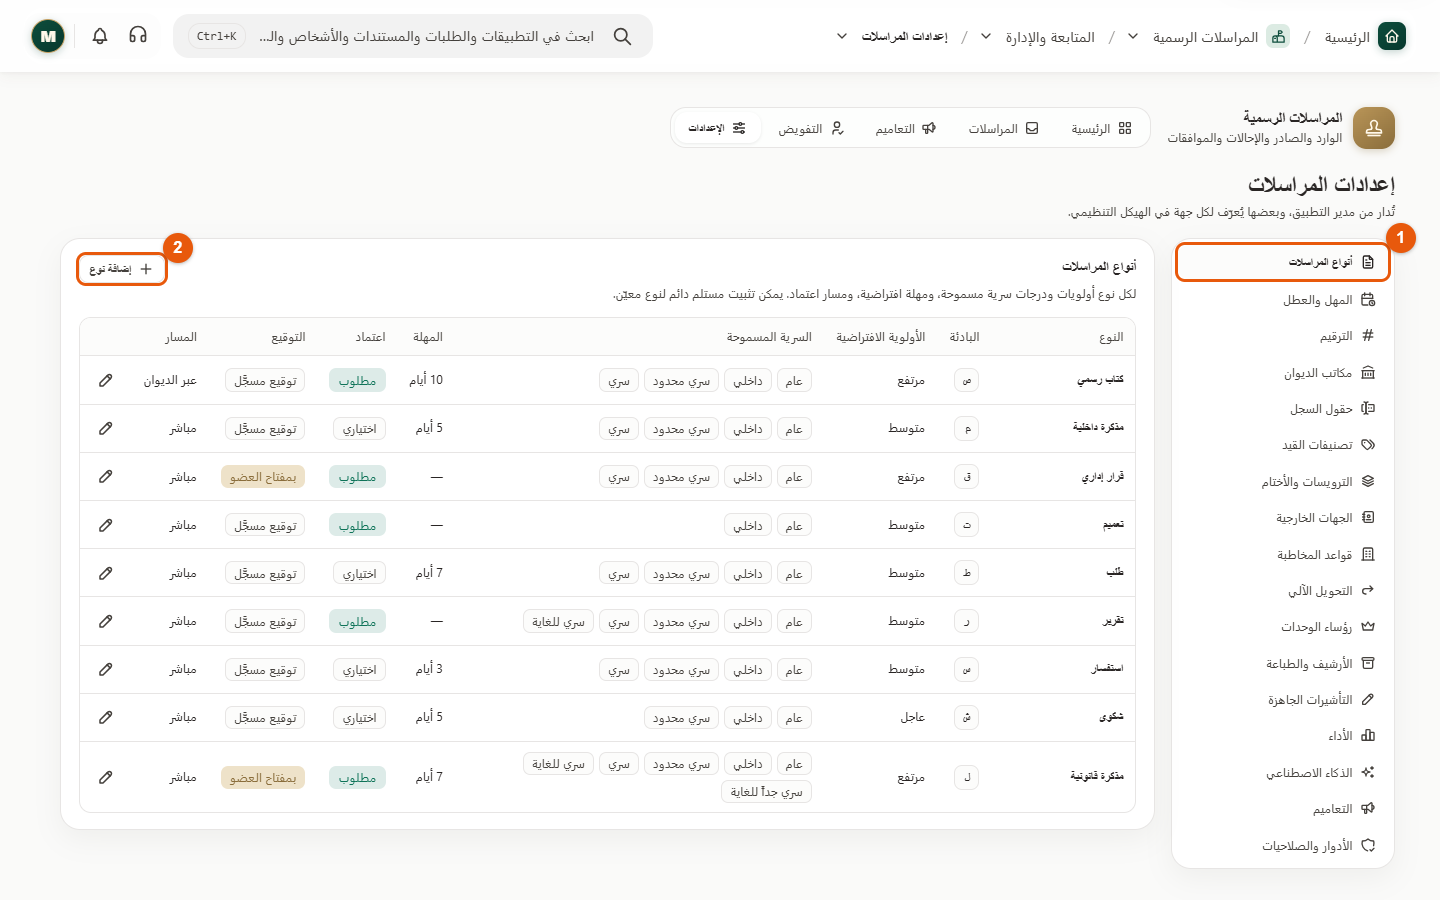
\includegraphics[width=0.95\linewidth]{assets/screens/org-correspondence-types.png}
\caption{ابدأ إعداد نوع الكتاب من قائمة الأنواع}
\label{fig:types-screen}
\shotnote{تساعدك القائمة على مقارنة المهلة والاعتماد والمسار قبل إنشاء النوع. الصورة تعرض الأنواع قبل إضافة نوع التدريب؛ قيم جدول التدريب هي التي سنكتبها. ① «أنواع المراسلات»: افتح هذا القسم. ② «إضافة نوع»: منه تبدأ إدخال القيم.}
\end{figure}

\section{جهّز شكل الورقة ودليل الجهات}
\label{sec:letterhead}
\textbf{لماذا؟} يجب أن يعرف المستلم من أرسل الكتاب، ويجب ألا نخلط بين وحدة داخل الوزارة وجهة خارجها. سنجهّز ترويسة الدائرة ونسجّل الفرن جهة خارجية لتمرين الرد.
\begin{enumerate}
\item افتح «الترويسات والأختام» ← «ترويسة جديدة». اكتب الاسم «ترويسة حماية المستهلك — تدريب»، وفي النص العربي: «وزارة الاقتصاد والصناعة» ثم «دائرة حماية المستهلك». وفي التذييل اكتب «نسخة تدريبية».
\item حدد «متاحة لـ» بما يشمل وحدة الدائرة أو مناصب الفريق، ثم «حفظ». من «ترويسات الوحدات» اضغط «إضافة وحدة» واربط الدائرة بالترويسة. لا تحتاج إلى تغيير افتراضية المؤسسة كلها.
\item اترك الختم فارغاً في أول تمرين. إذا احتجت إلى ختم معتمد، افتح «ختم جديد»، وحدد اسمه ووحدته و«المناصب المخوّلة» و«افتراضي عند»، وارفع الصورة المعتمدة ثم «حفظ». صورة الختم وحدها ليست قرار اعتماد.
\item افتح «الجهات الخارجية» ← «جهة جديدة». اكتب «فرن الأمانة» واختر النوع المناسب من القائمة ثم «حفظ». اترك البريد فارغاً في التدريب الورقي، ولا تخترع عنواناً لبريد حقيقي.
\item افتح «قواعد المخاطبة» وراجع قاعدة الدائرة. إذا كانت «مقيّدة»، أضف الفرن إلى الجهات المسموحة واحفظ. لا توسع قاعدة المؤسسة كلها من أجل هذا التمرين.
\end{enumerate}
\textbf{تحقق:} يظهر الفرن في دليل الجهات، وتظهر ترويسة الدائرة في مسودة جديدة. سجل الفرن في «المنشآت التجارية» والجهة الخارجية في المراسلات شيئان مختلفان؛ وجود الأول لا يعني إعداد الثاني تلقائياً.

\section{ادخل بصفتك واعرف أين تجد عملك}
\label{sec:mailbox}
\textbf{لماذا؟} قد تملك أكثر من منصب. فتح الصندوق بصفة مختلفة هو سبب شائع لغياب الكتاب أو زر الإجراء.
\begin{enumerate}
\item ادخل بحساب نور، وافتح تطبيق «المراسلات الرسمية» ثم «صندوق المراسلات».
\item افتح «أعمل بصفتي»، واختر «باحث ميداني — 01». اقرأ الصفة مرة أخرى قبل إنشاء الكتاب.
\item افتح «المسودات ومهام الصياغة» لتعرف أين ستعود إلى المسودة. ثم تعرّف إلى «بانتظار اعتمادي» و«الاستفسارات» دون إنشاء شيء.
\item إذا كانت قائمة فارغة، امسح البحث والتصفية وافحص الصفة. الفراغ قد يعني أنه لا يوجد عمل لك في هذه المرحلة.
\end{enumerate}
\begin{table}[H]
\centering
\caption{مكان العمل بحسب ما ينتظرك}
\label{tab:folders}
\begin{tabularx}{\linewidth}{R{4cm} Y}
\rcHeaderRow
\thh{المكان} & \thh{متى تفتحه؟}\\
المسودات ومهام الصياغة & لتكمل كتاباً لم يصدر بعد.\\
بانتظار اعتمادي & عندما تصل إليك مرحلة مراجعة أو اعتماد أو توقيع.\\
الاستفسارات & لتجيب عن سؤال موجّه إليك، لا لتجد كل سؤال أرسلته أنت.\\
ديوان الهيئة & للقيد وإرسال الصادر الخارجي ومتابعة السجلات.\\
الأرشيف & لمراجعة سجلات الأرشفة واعتمادها بحسب صلاحيتك.\\
\end{tabularx}
\end{table}
\textbf{تحقق:} اذكر اسم المنصب الظاهر في الصندوق. يجب أن يكون منصب نور، لا اسم أحمد ولا اسم المستخدم فقط.

\begin{figure}[H]
\centering
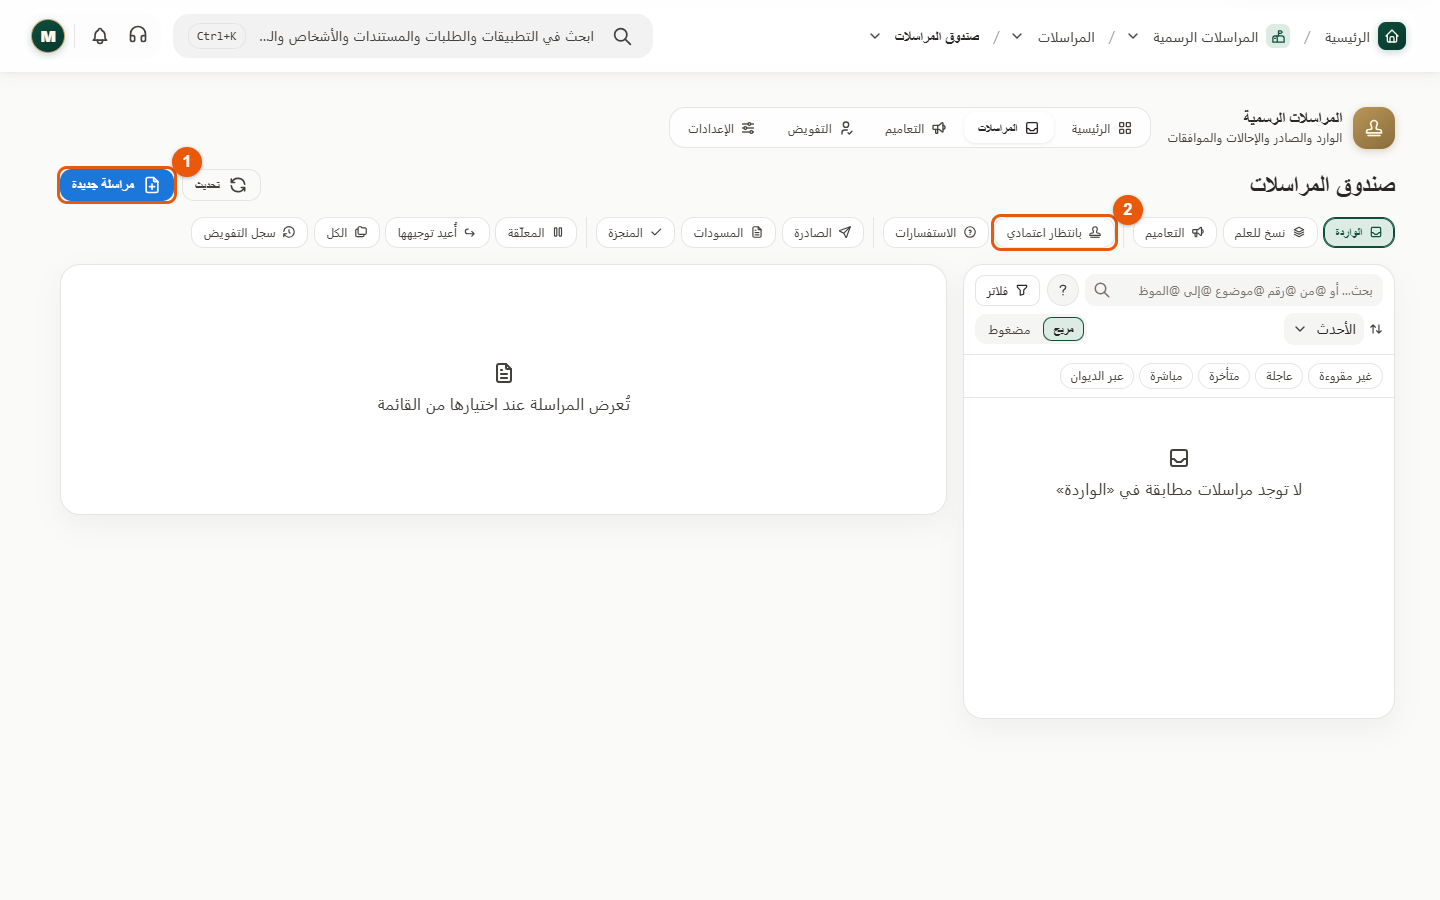
\includegraphics[width=0.95\linewidth]{assets/screens/org-correspondence-tray.png}
\caption{موضع إنشاء الكتاب ومجلد الاعتماد}
\label{fig:tray-screen}
\shotnote{الصندوق هنا فارغ؛ تعرفك الصورة بالأزرار ولا تعرض كتاباً منجزاً. اختيار الكتاب من القائمة يفتحه في مساحة القراءة. ① «مراسلة جديدة»: لبدء الكتاب. ② «بانتظار اعتمادي»: لما وصل دوره إلى منصبك.}
\end{figure}

\section{اكتب أول مسودة كاملة}
\label{sec:compose}
\textbf{لماذا؟} الموضوع يساعد على البحث، والنص يحدد المطلوب، والمخاطَب يحدد من سيعالج الكتاب بعد صدوره. نكتب طلباً واضحاً قبل إعداد مسار الموافقة.
\begin{enumerate}
\item بحساب نور وصفة الباحث اضغط «مراسلة جديدة».
\item اختر النوع «تنسيق كشف منشأة — تدريب»، والسرية «عام»، والأولوية «متوسط»، ولغة الكتاب العربية، وترويسة الدائرة.
\item اكتب في «الموضوع»: «تحديد موعد كشف على فرن الأمانة — تدريب 01».
\item اختر «تحرير النص»، واكتب النص المقترح أدناه. بدّل الموعد بموعد تدريبي واضح في المستقبل قبل الإرسال.
\item في «المخاطَبون» ← «إلى»، ابحث عن «رئيس فريق الكشف الميداني — 01» واختر نتيجة نوعها «منصب». اترك «نسخة للعلم» فارغة في أول دورة.
\item اقرأ «مسار التوجيه المتوقع». لا تفعّل «إرسال مباشر دون المرور بالديوان» في هذا التمرين؛ المسار المباشر له شروط منها كتاب داخلي ومستلم واحد.
\end{enumerate}
\begin{rcnote}[نص جاهز للتطبيق]
إلى رئيس فريق الكشف الميداني، نرجو تحديد موعد للكشف على فرن الأمانة خلال أسبوع العمل القادم، وتسمية المسؤول عن تنسيق الزيارة. سأجهّز قائمة بيانات المنشأة قبل الموعد. يرجى إبلاغي بالموعد المعتمد حتى أستكمل التحضير. مع الشكر.
\end{rcnote}
\begin{table}[H]
\centering
\caption{لا تخلط بين هذه الحقول}
\label{tab:compose}
\begin{tabularx}{\linewidth}{R{3.5cm} Y}
\rcHeaderRow
\thh{الحقل} & \thh{ما الذي نضعه فيه؟}\\
الموضوع & \req{} عنوان واضح من خمسة أحرف على الأقل؛ لا تكتب «هام» فقط.\\
إلى & \req{} من سيعالج الكتاب؛ أحمد في المثال.\\
نسخة للعلم & \opt{} من يحتاج معرفة النتيجة دون تكليفه بعمل.\\
مسار الاعتماد & من يراجع ويوقّع قبل وصول الكتاب إلى المخاطَب؛ نضبطه تالياً.\\
الأولوية والسرية & الاستعجال مختلف عن تقييد الاطلاع؛ لا ترفع السرية لمجرد أن الكتاب عاجل.\\
\end{tabularx}
\end{table}
\textbf{تحقق:} ترى الموضوع والنص واسم المنصب المخاطَب في الورقة. لا تعتمد على تشابه أسماء الأشخاص؛ اختر المنصب الكامل.

\begin{figure}[H]
\centering
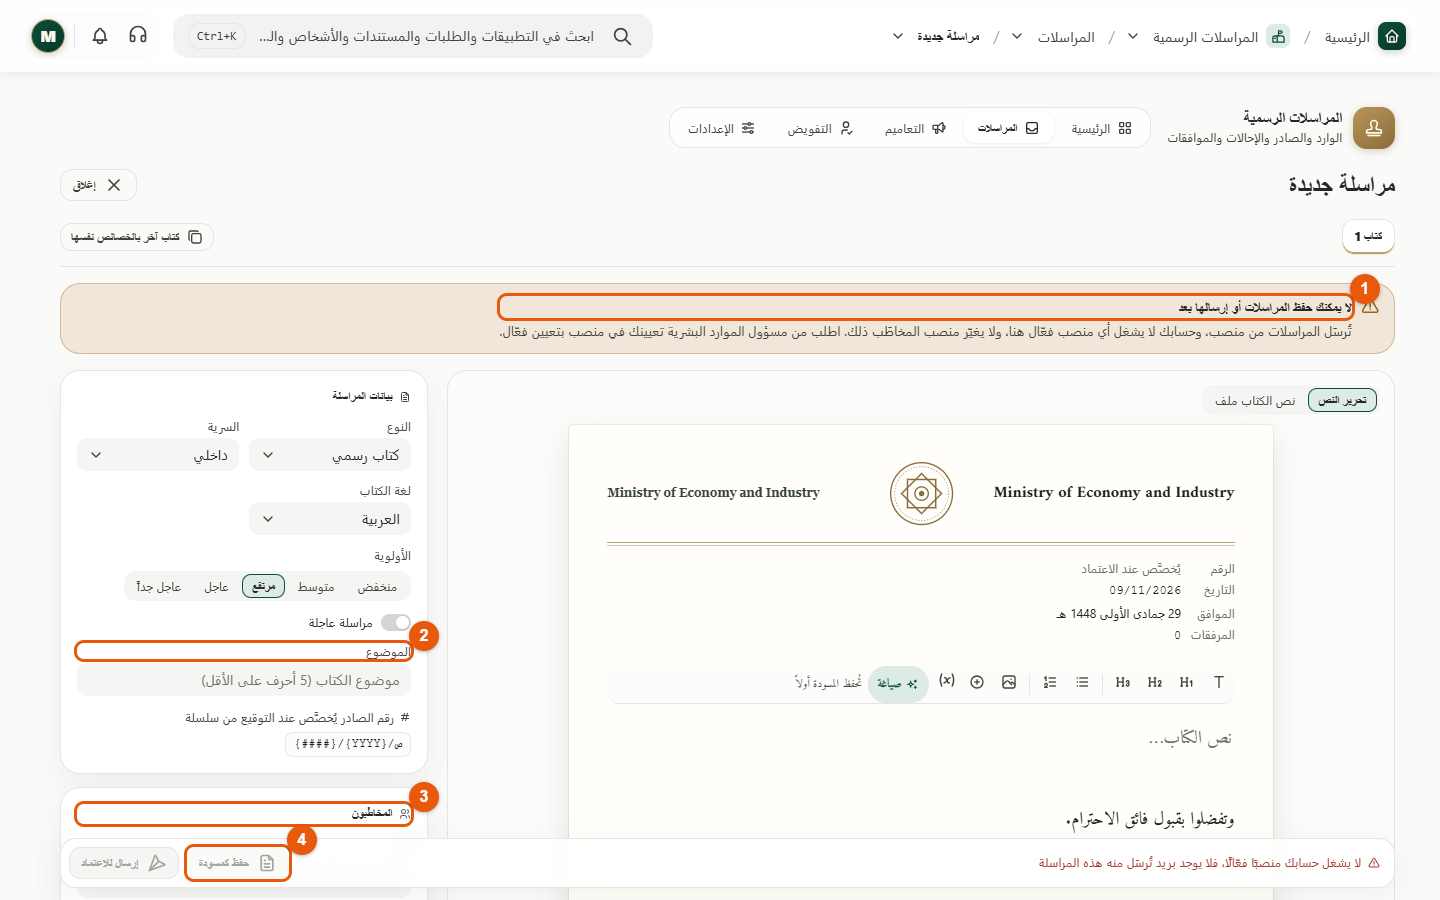
\includegraphics[width=0.95\linewidth]{assets/screens/org-correspondence-compose.png}
\caption{تعرّف إلى الحقول وحالة غياب المنصب}
\label{fig:compose-screen}
\shotnote{هذه حالة قبل إكمال المتطلبات، وليست مسودة محفوظة: الحساب بلا منصب فعّال، لذلك الحفظ والإرسال غير متاحين. عالج التعيين أولاً، ثم أدخل قيم تمريننا بدلاً من القيم الابتدائية الظاهرة. ① تنبيه غياب المنصب. ② «الموضوع». ③ «المخاطَبون». ④ «حفظ كمسودة»: تستخدمه بعد اكتمال المتطلبات.}
\end{figure}

\section{حدد من يراجع ومن يوقّع}
\label{sec:approval-route}
\textbf{لماذا؟} اختيار ريم في «إلى» لا يجعلها مراجعة. يجب وضعها في مسار الاعتماد إذا أردنا أن تقرأ الكتاب قبل صدوره.
\begin{enumerate}
\item في المسودة افتح «مسار الاعتماد». احفظ المسودة أول مرة إذا كانت الواجهة تنتظر الحفظ لاقتراح المسار.
\item اقرأ المراحل المقترحة. لا تفترض أنها مطابقة لفريقنا؛ فقد تُستنتج من رئيس الوحدة ومرجعه.
\item جهّز مسار التدريب بمرحلتين عبر «إضافة مرحلة»: منصب «مدقق كشوف المنشآت — 01» بدور «مراجعة»، ثم «رئيس فريق الكشف الميداني — 01» بدور «توقيع». أزل المراحل الزائدة المسموح بإزالتها وتحقق من الترتيب.
\item إذا فرض النوع أو سياسة المؤسسة مساراً لا يسمح بهذا التعديل، يضبطه المسؤول قبل المتابعة؛ لا ترسل مساراً مختلفاً وتنتظر وصوله إلى ريم.
\item احفظ المسودة وأعد فتحها، واقرأ ترتيب المراحل مرة ثانية.
\end{enumerate}
\begin{rcnote}[نفس المنصب في وظيفتين]
أحمد هنا موقّع ومخاطَب في الوقت نفسه: يوقّع بصفته صاحب المرحلة، ثم يعالج الطلب بصفته المستلم. انتهاء التوقيع لا يعني أن عمل المستلم أُنجز. لاحقاً سنرى العمل المفتوح في «المسار».
\end{rcnote}
\textbf{تحقق:} تستطيع قراءة المسار بصوت واضح: نور يُعدّ، ريم تراجع، أحمد يوقّع، ثم أحمد يعالج الطلب. «نسخة للعلم» ليست مرحلة موافقة.

\begin{figure}[H]
\centering
\begin{tikzpicture}[node distance=0.5cm]
\node[stepBox] (a) {\RL{نور: إعداد المسودة}};
\node[stepBox,below=of a] (b) {\RL{ريم: مراجعة الكتاب}};
\node[stepBox,below=of b] (c) {\RL{أحمد: التوقيع والإصدار}};
\node[stepBox,below=of c] (d) {\RL{المستلم: معالجة ثم إنجاز}};
\draw[flowsTo] (a) -- (b);
\draw[flowsTo] (b) -- (c);
\draw[flowsTo] (c) -- (d);
\end{tikzpicture}
\rclegend
\caption{مسار الكتاب الداخلي في التدريب}
\label{fig:internal-route}
\shotnote{رسم توضيحي لتسلسل المسؤوليات. عند الإعادة يرجع الكتاب إلى نور ليعدّله ويعيد إرساله. معالجة المستلم تبدأ بعد الإصدار، ولا تنتهي لمجرد التوقيع.}
\end{figure}

\section{أضف المرفق واحفظ ثم أعد الفتح}
\label{sec:save}
\textbf{لماذا؟} ظهور النص على الشاشة لا يثبت وصوله إلى الحفظ. سنضيف مرفقاً ونختبر استرجاعه، قبل إرسال الكتاب لأي مرحلة.
\begin{enumerate}
\item جهّز ملفاً تدريبياً بعنوان «بيانات فرن الأمانة» يحتوي اسم الفرن والغرض من الزيارة فقط. من «المرفقات والمراجع» اضغط «اختيار ملف» وارفعه، ثم انتظر اكتمال الرفع.
\item راجع الورقة: الموضوع، المخاطَب، النص، الترويسة، وعدد المرفقات. إذا ذكرت مرفقاً في النص، تأكد أنه مرفوع فعلاً.
\item اضغط «فحص الآن»، واقرأ الملاحظات وأصلح ما ينطبق. الفحص مساعد للمراجعة وليس اعتماداً، ونتيجة فحص القواعد وحدها ليست مراجعة لغوية كاملة.
\item اضغط «حفظ كمسودة». افتح «المسودات ومهام الصياغة»، وابحث عن «تدريب 01»، وافتح المسودة ثانية.
\item اقرأ النص وافتح المرفق وتأكد من مسار الاعتماد. لا ترسل بعد؛ سنجرّب الإعادة للتعديل في الخطوة التالية.
\end{enumerate}
\begin{table}[H]
\centering
\caption{الحفظ والملفات}
\label{tab:save}
\begin{tabularx}{\linewidth}{R{4cm} Y}
\rcHeaderRow
\thh{ما يظهر أو ما تختاره} & \thh{كيف تتصرف؟}\\
تغييرات غير محفوظة & انتظر الحفظ أو اضغط «حفظ كمسودة».\\
تعذّر الحفظ & اقرأ السبب؛ لا تغادر وتفترض أن الحفظ التلقائي نجح.\\
المرفقات & حتى عشرة ملفات، وحتى 20 ميغابايت لكل ملف، من الأنواع التي تقبلها النافذة.\\
نص الكتاب ملف & بديل لتحرير النص: ملف PDF أو Word حتى 20 ميغابايت. ليس مجرد مرفق إضافي. راجع مناطق الترويسة والتوقيع المطلوبة في القالب.\\
الحفظ التلقائي & يبدأ عند اكتمال الموضوع والمخاطَبين، وليس ضماناً لحفظ كتاب ناقص.\\
\end{tabularx}
\end{table}
\textbf{تحقق:} أغلقت المسودة وأعدت فتحها فوجدت النص والمخاطَب والمرفق والمراحل. هذه أول نتيجة عملية، وليست مجرد رسالة نجاح.

\section{أرسل للمراجعة وجرّب إعادة الكتاب للتعديل}
\label{sec:return}
\textbf{لماذا؟} الإعادة تسمح بتصحيح كتاب صالح في أصله. سنتعلمها قبل التوقيع حتى لا نبحث عن تعديل نص صار نهائياً.
\begin{enumerate}
\item بحساب نور افتح المسودة المحفوظة، وتأكد من أن أول مرحلة لريم. اضغط «إرسال للاعتماد» وأكّد بعد قراءة نافذة التأكيد.
\item بحساب ريم اختر صفة «مدقق كشوف المنشآت — 01» وافتح «بانتظار اعتمادي»، ثم كتاب «تدريب 01».
\item اقرأ النص والمرفق. اضغط «إعادة للتعديل» واكتب «يرجى تحديد يوم الزيارة والوقت المقترح بوضوح»، ثم أكّد الإعادة.
\item عد بحساب نور إلى الكتاب المُعاد. اقرأ الملاحظة، وأضف إلى النص موعداً تدريبياً محدداً، ثم احفظ وأعد الإرسال.
\item عد بحساب ريم وافتح «بانتظار اعتمادي» وتحقق من وجود النص المعدّل. يبدأ المسار من جديد بعد إعادة الإرسال.
\end{enumerate}
\begin{rcnote}[لا تستخدم الرفض لتصحيح كلمة]
«رفض» ينهي مسار الكتاب ولا يعيده إلى التعديل والإرسال. استخدم «إعادة للتعديل» عندما تكون الفكرة مقبولة وتحتاج استكمالاً. اكتب ملاحظة واضحة من خمسة أحرف على الأقل؛ «ناقص» وحدها لا تشرح ما المطلوب.
\end{rcnote}
\textbf{تحقق:} رأى نور سبب الإعادة، وعدّل الموعد، ووصلت النسخة الجديدة إلى ريم. إن لم يظهر الكتاب، افحص صفتها والمرحلة الحالية، ثم امسح التصفية.

\section{اعتمد ووقّع وافحص النتيجة}
\label{sec:sign}
\textbf{لماذا؟} مراجعة ريم تنهي مرحلتها فقط. توقيع أحمد هو الخطوة التي تُصدر الكتاب وتثبت نصه ورقمه.
\begin{enumerate}
\item بحساب ريم اقرأ النص المعدّل والمرفق، ثم اضغط «اعتماد» وأكّد. راقب انتقال الدور إلى أحمد.
\item بحساب أحمد اختر صفة رئيس الفريق وافتح «بانتظار اعتمادي». تأكد أن الكتاب ينتظر توقيعه وأن ريم أنهت مرحلتها.
\item اضغط «اعتماد وتوقيع». اقرأ الرقم المتوقع والختم إن وُجد وحاشية الاعتماد. لا تكتب الرقم المتوقع في سجل خارجي؛ الرقم النهائي يُحجز عند التنفيذ.
\item أكّد التوقيع. افتح الكتاب الصادر واقرأ رقمه الفعلي، وسجّل الرقم في ملاحظات التدريب.
\item افحص النص والترويسة والمسار والتوقيع. انتقل إلى عمل أحمد كمستلم لترى الطلب الذي يحتاج معالجة.
\end{enumerate}
\textbf{تحقق:} اختفى الكتاب من انتظار توقيع أحمد، وحمل رقماً، وثبت نصه، وظهر عمل المستلم في المسار. إذا طلب النظام مفتاح توقيع، جهّز المفتاح المطلوب أو راجع إعداد النوع مع المسؤول؛ لا تُعدّ صورة التوقيع بديلاً عنه.

\section{اختم الكتاب الداخلي بقرار واضح}
\label{sec:complete}
\textbf{لماذا؟} صدر طلب نور لكن تحديد الموعد ما زال عملاً لدى أحمد. نريد إغلاقه بنتيجة مفهومة لمن يعود إلى الكتاب لاحقاً.
\begin{enumerate}
\item بحساب أحمد افتح الكتاب من صندوقه بصفته المستلم، واقرأ «المسار» لمعرفة العمل المفتوح لديه.
\item إذا كان المطلوب جواباً رسمياً، اضغط «رد» وأنشئ كتاباً مرتبطاً بالأصل، وأكمل اعتماده حتى يصدر. مجرد حفظ الرد لا يغلق العمل.
\item في تمريننا الأول يكفي تسجيل اعتماد الموعد: اضغط «إنجاز وحفظ»، واكتب «تم تحديد موعد الكشف وفق الموعد المذكور في الكتاب، وسيجهز نور بيانات المنشأة».
\item راجع «الحفظ في الأرشيف» ثم أكّد «إنجاز وحفظ». النسخة الرسمية تُحفظ دائماً؛ اختيار مكان إضافي لا يستبدلها.
\item افتح المسار مرة أخرى. إذا بقيت المراسلة «قيد المعالجة»، ابحث عن عمل مفتوح أو معلّق لجهة أخرى، ولا تكرر الإنجاز عشوائياً.
\end{enumerate}
\textbf{تحقق:} ترى حاشية الإنجاز وانتهاء عمل أحمد. لو كان لديه مجرد نسخة للعلم، لكان الإجراء «إقرار بالاطلاع»، وليس «إنجاز وحفظ».

\section{تعلّم مراجعة الصياغة في مسودة منفصلة}
\label{sec:drafting}
\textbf{لماذا؟} «دفع للمراجعة» قبل الاعتماد ليس هو وضع ريم في مسار الاعتماد. قبوله ينقل ملكية المسودة إلى المراجِع، لذلك سنجرّبه في كتاب مستقل كي لا نغيّر قصة كتابنا الأول.
\begin{enumerate}
\item بحساب نور أنشئ مسودة بعنوان «مراجعة صياغة تقرير فرن الأمانة — تدريب 02»، وضع أحمد مخاطَباً، واكتب ملخصاً قصيراً واحفظ.
\item اضغط «دفع للمراجعة». اختر منصب ريم في «المراجِع»، واكتب «يرجى تدقيق وضوح المطلوب والموعد ثم إعادة المسودة مع الملاحظات»، وأكّد الدفع.
\item بحساب ريم افتح «مهام الصياغة» ← «المُسندة إليّ». افتح الطلب واضغط «إعادة»، واكتب «يرجى ذكر الموعد المحدد بدلاً من عبارة قريباً».
\item بحساب نور افتح «التي أسندتُها»، واقرأ الملاحظة ثم عدّل المسودة. إذا أردت تجربة «قبول»، ادفعها ثانية، ثم تقبلها ريم وتفحصان المالك والمسار الجديدين.
\end{enumerate}
\begin{table}[H]
\centering
\caption{قرارات مهمة الصياغة}
\label{tab:drafting}
\begin{tabularx}{\linewidth}{R{3cm} Y}
\rcHeaderRow
\thh{القرار} & \thh{النتيجة}\\
قبول & تصبح المسودة ملك منصب المراجِع، ويُحسب المسار الافتراضي من منصبه؛ لا يصدر الكتاب.\\
إعادة & تعود المسودة إلى مُعدّها مع ملاحظات الإعادة.\\
سحب & يُنهي طالب المراجعة الطلب ويستعيد إمكانية التحرير.\\
إلغاء & يُنهي أحد الطرفين الطلب وتبقى المسودة لدى صاحبها.\\
\end{tabularx}
\end{table}
\textbf{تحقق:} أثناء انتظار المراجعة كانت المسودة مقفلة للتحرير. بعد الإعادة يستطيع نور تعديلها. بعد القبول لا تتوقع أن تبقى ضمن مسودات نور؛ يتابع طلبه من «التي أسندتُها».

\section{استقبل كتاباً ورقياً دون منحه رقماً بعد}
\label{sec:paper}
\textbf{لماذا؟} قد تصل صورة كتاب قبل اكتمال بياناته. نحفظها في انتظار القيد، ثم نراجعها قبل توزيعها رسمياً.
\begin{enumerate}
\item جهّز ورقة تدريبية بعنوان «طلب استكمال كشف فرن الأمانة — تدريب 03»، باسم الجهة المرسلة «فرن الأمانة»، ورقم مرسل تجريبي \en{TRAIN-03}، وتاريخ اليوم، ونص يطلب بيان النواقص المطلوبة لاستكمال الكشف. احفظها PDF أو صورة واضحة.
\item بحساب أحمد افتح «ديوان الهيئة» ثم «قيد وارد ورقي». ارفع الورقة في «الصورة والمرفقات»، وأدخل الموضوع ورقم المرسل والبيانات المتوفرة.
\item إذا اخترت «الموجَّه إليه»، اختر منصب رئيس الفريق؛ هذا يساعد على التوزيع لاحقاً ولا يسلّم الكتاب الآن.
\item اضغط «حفظ بانتظار القيد»، ثم افتح «بانتظار القيد» وابحث عن «تدريب 03».
\item افتح الصورة وراجع وضوح الصفحات. إذا استعملت «قيد بالمسح الضوئي»، قارن البيانات المستخرجة بالورقة حرفاً حرفاً، خصوصاً رقم المرسل وتاريخه؛ يمكنك الإدخال يدوياً عند تعذر القراءة.
\end{enumerate}
\textbf{تحقق:} تظهر بطاقة الوارد في الانتظار، ولا يحصل الكتاب على رقم وارد بعد. رقم \en{TRAIN-03} هو رقم المرسل، وليس رقم قيد الدائرة.

\section{قيّد الوارد ووزّعه على صاحب العمل}
\label{sec:incoming}
\textbf{لماذا؟} الآن نحول الصورة إلى مراسلة رسمية مرقّمة. نرسلها إلى أحمد للإجراء، ليحيلها في الخطوة التالية إلى نور.
\begin{table}[H]
\centering
\caption{بيانات القيد لهذا الوارد}
\label{tab:incoming}
\begin{tabularx}{\linewidth}{R{3.7cm} Y}
\rcHeaderRow
\thh{الحقل} & \thh{القيمة وسببها}\\
تصنيف القيد & وارد؛ يحدد السلسلة المستخدمة.\\
الجهة المرسلة & \req{} فرن الأمانة.\\
الموضوع & \req{} طلب استكمال كشف فرن الأمانة — تدريب 03.\\
تاريخ الورود & تاريخ وصول الكتاب الفعلي؛ لا تختَر تاريخاً مستقبلياً.\\
نوع المراسلة والسرية والأولوية & نوع التدريب، «عام»، «متوسط».\\
يوزَّع إلى & \req{} رئيس فريق الكشف الميداني — 01، والغرض «للإجراء».\\
رداً على كتابنا رقم & \opt{} فارغ هنا؛ هذا وارد جديد، وليس رداً على كتاب صادر سابق.\\
حاشية الديوان & \rec{} «لبيان النواقص المطلوبة لاستكمال الكشف».\\
\end{tabularx}
\end{table}
\begin{enumerate}
\item على بطاقة «تدريب 03» اضغط «قيد وتوزيع». راجع قيم الجدول والمرفقات. لا تبدأ قيداً آخر للورقة نفسها.
\item اختر منصب أحمد في «يوزَّع إلى» وحدد «للإجراء». لو اخترت «للاطلاع» فلن تطلب منه معالجة الوارد.
\item اقرأ المهلة والرقم المتوقع ثم اضغط «قيد وتوزيع». انتظر اكتمال الحفظ وانتهاء مهلة التراجع قبل التحقق من وصول الإشعار.
\item انسخ الرقم النهائي من نتيجة القيد إلى ملاحظات التدريب. ابحث عنه في «سجل الوارد» ثم افتحه من صندوق أحمد.
\item إذا كان للكتاب أصل ورقي تسلّمه أحد، استخدم «إجراءات القيد» ← «تسليم الأصل الورقي» وسجّل التسليم الفعلي. تسجيل الصورة لا يثبت تسليم الأصل.
\end{enumerate}
\textbf{تحقق:} ترى قيداً واحداً برقم وارد وموضوع صحيح، وعمل إجراء مفتوحاً لدى أحمد. إذا ظهر تحذير رقم مكرر، ابحث عن القيد السابق قبل إعادة الحفظ. وإذا تراجعت عن قيد، يبقى رقمه ملغى ولا يُعاد استخدامه.

\section{أحل الوارد إلى نور مع توجيه ومهلة}
\label{sec:refer}
\textbf{لماذا؟} أحمد يتابع الطلب، ونور يجمع النواقص ويجهّز الجواب. الإحالة تنقل العمل إليه وتبقي نتيجة الإنجاز قابلة للمتابعة.
\begin{enumerate}
\item بحساب أحمد افتح الوارد المرقّم ثم اضغط «إحالة».
\item اختر منصب «باحث ميداني — 01»، واجعل الغرض «للإجراء». اكتب الحاشية: «يرجى مراجعة بيانات فرن الأمانة وإعداد بيان بالنواقص المطلوبة لاستكمال الكشف».
\item حدد «مهلة الإنجاز للمحال إليهم» بخمسة أيام عمل في التمرين. اترك «إخفاء الحواشي السابقة عن المحال إليهم» غير مفعّل حتى يقرأ نور التوجيه السابق.
\item أكّد «إحالة». افتح «المسار» لترى انتقال العمل إلى نور.
\item بحساب نور افتح الوارد واقرأ الورقة والحاشية والمهلة. لا تبدأ العمل اعتماداً على عنوان الإشعار وحده.
\end{enumerate}
\begin{rcnote}[متى أستخدم الحاشية أو إعادة التوجيه؟]
إذا أردت التعليق فقط، استخدم «حاشية». إذا وصل إليك العمل بالخطأ وتريد تسليمه إلى الجهة الصحيحة دون انتظار نتيجته عندك، استخدم «إعادة توجيه» عندما تكون متاحة. أما «إحالة» للإجراء فتُبقيك متابعاً لنتيجة من أحلت إليه. إحالة للاطلاع فقط لا تنقل عملك.
\end{rcnote}
\textbf{تحقق:} يرى نور عملاً مفتوحاً، ويرى أحمد محطة الإحالة واسم المنصب والمهلة. لا يكفي أن تظهر حاشية أحمد؛ يجب أن يظهر انتقال العمل أيضاً.

\section{اطلب إفادة عندما تنقصك معلومة}
\label{sec:inquiry}
\textbf{لماذا؟} نور يحتاج من ريم تحديد النواقص التي يجب ذكرها في الرد. الاستفسار يحفظ السؤال والإجابة مع الكتاب، بدلاً من ترك القرار في محادثة منفصلة.
\begin{enumerate}
\item بحساب نور ومن الوارد اضغط «استفسار». اختر منصب ريم، واكتب «هل النقص المطلوب في هذا التدريب هو عنوان المنشأة التفصيلي فقط؟»، ثم «إرسال الاستفسار».
\item بحساب ريم افتح «الاستفسارات»، ثم الكتاب، واضغط «إفادة». اكتب «نعم، المطلوب في هذا التدريب استكمال العنوان التفصيلي قبل متابعة الكشف»، ثم «إرسال الإفادة».
\item عد بحساب نور إلى الكتاب نفسه واقرأ الإفادة في سياقه. لا تبحث عن سؤالك الصادر في مجلد الأسئلة الموجهة إليك.
\item إذا طرحت السؤال بالخطأ ولم تعد تحتاجه، استخدم «إلغاء الاستفسار» مع الحفاظ على فهم سبب الإلغاء.
\end{enumerate}
\textbf{تحقق:} زال انتظار الإفادة، وسُجل السؤال والجواب. الاستفسار المفتوح يمنع إنهاء عمل صاحبه وإعادة توجيهه، وقد يوقف الاعتماد والتوقيع إذا طرحه صاحب المرحلة أثناء الاعتماد.

\section{اكتب رداً مرتبطاً بالوارد وأصدره}
\label{sec:reply}
\textbf{لماذا؟} نريد أن نجد طلب الفرن والجواب عليه معاً. «رد» ينشئ الرابط، أما كتابة كتاب مستقل بالعنوان نفسه فلا تكفي.
\begin{enumerate}
\item بحساب نور افتح الوارد واضغط «رد». راجع مرجع الكتاب الأصلي في المسودة الجديدة.
\item اكتب الموضوع «استكمال عنوان فرن الأمانة لإتمام الكشف — تدريب 03». وفي النص اكتب: «إشارة إلى كتابكم المحفوظ برقم الوارد المذكور في المرجع، يرجى تزويد دائرة حماية المستهلك بعنوان المنشأة التفصيلي لاستكمال إجراءات الكشف. مع الشكر».
\item افحص «إلى» وتأكد أن الجهة الخارجية هي «فرن الأمانة» من الدليل؛ لا تفترض أن الجهة المقترحة صحيحة دون قراءتها.
\item اختر نوع التدريب والترويسة، ورتب مسار ريم للمراجعة ثم أحمد للتوقيع، وأضف المرفقات المطلوبة فقط. احفظ ثم افتح المسودة ثانية.
\item أرسلها إلى الاعتماد. تعتمد ريم مرحلتها ثم يوقّع أحمد كما فعلتما في الكتاب الأول. سجّل رقم الصادر النهائي.
\item افتح الوارد الأصلي وافحص انتهاء عمل نور المرتبط بالرد، ثم افتح الصادر وافحص مرجعه وحالة إرساله الخارجي.
\end{enumerate}
\textbf{تحقق:} يظهر رابط بين الأصل والرد، وللرد رقم صادر. إنجاز عمل نور بصدور الرد لا يثبت تسليم الجواب إلى الفرن؛ سنفحص الإرسال في الخطوة التالية.

\section{أرسل الصادر وسجّل التسليم الحقيقي}
\label{sec:dispatch}
\textbf{لماذا؟} الكتاب الخارجي الموقّع ينتظر في الديوان. الإصدار يثبت محتواه، والإرسال يثبت خروجه، والتسليم يثبت وصوله بحسب الوسيلة والإثبات المتوفر.
\begin{enumerate}
\item بحساب أحمد افتح «ديوان الهيئة» ← «بانتظار الإرسال». ابحث عن رقم الرد على الفرن، وافتحه للتأكد من الجهة والمرفقات.
\item اضغط «تسجيل الإرسال» واقرأ «وسيلة الإرسال». في التدريب الورقي، اختر الوسيلة الورقية المتاحة وسجّل الإجراء بعد تسليم النسخة في المحاكاة التدريبية، ثم «تأكيد الإرسال». لا تسجل وصولاً لم يحدث.
\item إن كان الإرسال بالبريد مطلوباً فعلاً، جهّز بريد الديوان وبريد الجهة الصحيح أولاً. اختيار «بريد إلكتروني» ثم «إرسال مباشر بالبريد» يرسل رسالة فعلية، وليس مجرد تغيير للحالة.
\item افتح «سجل الصادر» وابحث عن الرقم، واقرأ بيانات الإرسال. إذا تعذّر الإرسال اقرأ السبب قبل إعادة المحاولة.
\end{enumerate}
\begin{rcnote}[رفض الإرسال ليس إلغاء رقم الكتاب]
إذا كانت حزمة الصادر غير صالحة للإرسال، يختار موظف الديوان «رفض الإرسال» مع سبب واضح لإبلاغ الجهة المرسِلة. لا تحاول تعديل نص موقّع من شاشة الإرسال. تصحيح أو إلغاء قيد أنشأه الديوان يختلف عن استرداد كتاب أصدره مرسله، ويجب استخدام الإجراء المناسب لحالة الكتاب.
\end{rcnote}
\textbf{تحقق:} ترى وسيلة الإرسال ونتيجته في السجل. لا تعتمد على اختفاء البطاقة وحده، ولا تعتبر رقم الصادر دليلاً على وصول البريد أو استلام الورقة.

\section{جرّب حقيبة إرسال عند وجود عدة كتب}
\label{sec:batch}
\textbf{لماذا؟} الحقيبة تجمع عدة كتب بقناة واحدة، وتتابع نتيجة كل كتاب. نفّذ هذه الخطوة على صادر تدريبي آخر لم تُسجل إرساله في الخطوة السابقة.
\begin{enumerate}
\item جهّز رداً تدريبياً ثانياً بالطريقة السابقة حتى يصبح بانتظار الإرسال، ثم افتح «حقائب الإرسال» ← «حقيبة جديدة».
\item اكتب الاسم «كتب حماية المستهلك — تدريب»، واختر القناة الورقية المتاحة، ثم «إنشاء الحقيبة».
\item اضغط «إضافة كتب»، وحدد الكتاب المؤهل الذي لم يُرسل، ثم «إضافة».
\item اضغط «تحقق من الأهلية». عالج سبب كل بند غير مؤهل قبل «إرسال الحقيبة»؛ البنود غير المؤهلة لا تخرج مع البقية.
\item اطبع الكشف من «طباعة الكشف». بعد محاكاة تسليم الورقة اضغط «تسليم» للبند وسجّل اسم المستلم التدريبي المعروف.
\end{enumerate}
\textbf{تحقق:} حالة البند الورقي «سُلّمت»، وليست مجرد «جاهزة للإرسال». قد تنتهي حقيبة متعددة الكتب جزئياً؛ اقرأ كل بند. وفي البريد ذي الإرسال غير المؤكد افحص مجلد المرسل قبل إعادة الإرسال لتجنب نسخة ثانية.

\section{أكمل دورة الوارد إذا وصل جواب جديد}
\label{sec:incoming-reply}
\textbf{لماذا؟} إذا طلبت معلومة من جهة خارجية، يجب ربط جوابها بالكتاب الصادر حتى يعرف الفريق أن انتظار الرد انتهى.
\begin{enumerate}
\item جهّز جواباً ورقياً تدريبياً من الفرن يذكر العنوان التفصيلي، ورقم مرسل جديداً \en{TRAIN-04}.
\item احفظه كوارِد ورقي ثم افتح «قيد وتوزيع». في «رداً على كتابنا رقم» ابحث عن رقم الصادر الفعلي الذي سجلته، واختره.
\item وزعه على منصب نور «للإجراء»، وراجع الجهة والموضوع والتاريخ ثم أكمل القيد.
\item بحساب نور افتح الوارد، وتحقق من اكتمال المعلومة، ثم سجّل نتيجة المعالجة باستخدام «إنجاز وحفظ» إذا لم تعد تحتاج إلى كتاب رد جديد.
\end{enumerate}
\textbf{تحقق:} يظهر جواب الفرن مرتبطاً بالصادر الصحيح وتتوقف متابعة انتظار الرد عليه. كتابة الرقم في نص الكتاب وحدها لا تعوّض اختيار المرجع في حقل الربط.

\section{اجمع القصة كاملة في إضبارة}
\label{sec:dossier}
\textbf{لماذا؟} أصبح لدينا طلب داخلي ووارد ورد وجواب. الإضبارة تجمع هذه السلسلة حتى يستطيع الفريق متابعة موضوع الفرن دون بحث منفصل كل مرة.
\begin{enumerate}
\item بحساب نور افتح «الأضابير» ← «إضبارة جديدة». اختر «دائرة حماية المستهلك»، واكتب «مراسلات كشف فرن الأمانة — تدريب»، ووصفاً يشرح أنها تجمع كتب هذا التمرين، ثم «فتح الإضبارة».
\item افتح كل كتاب يحق لنور قراءته، ثم «إجراءات أخرى» ← «إضافة إلى إضبارة». اختر الإضبارة واضغط «إضافة».
\item افتح الإضبارة وتأكد من ظهور الكتب وأرقامها. اضغط «مشاركة» وأضف منصبي أحمد وريم، وحدد من يحتاج «صلاحية الإدارة» ثم «حفظ».
\item بحساب ريم افتح الإضبارة. إذا ظهر كتاب «مراسلة مقيّدة»، فالمشاركة لا تمنحها محتواه. يتولى صاحب الحق «منح اطلاع» وفق صلاحيات الكتاب عند الحاجة.
\item لا تضغط «إغلاق الإضبارة» إلا بعد اكتمال كل الموضوع؛ الإغلاق نهائي لا رجوع عنه. إن أضفت كتاباً خطأ استخدم «إزالة» من الإضبارة، وهي لا تحذف الكتاب.
\end{enumerate}
\textbf{تحقق:} تستطيع الوصول من الإضبارة إلى الوارد والرد، ومن الكتاب إلى «ضمن الأضابير». عدد الكتب وحده لا يثبت أن كل مشارك يستطيع قراءة محتواها.

\section{أرسل تعميماً محدوداً وتابع الإقرار}
\label{sec:circular}
\textbf{لماذا؟} التعميم مناسب لتعليمات واحدة تصل إلى جمهور محدد، مثل قائمة البيانات المطلوبة قبل الكشف. لا نحتاج إلى توجيه التمرين إلى جميع العاملين.
\begin{enumerate}
\item بحساب المسؤول تأكد من وجود نوع مناسب للتعميم ومسار توقيعه، وامنح منصب الناشر صلاحية «نشر التعاميم» من «إدارة الأدوار». تسمي صفحة الشرح هذا الدور «ناشر التعاميم». ثم بحساب المُعدّ افتح «مراسلة جديدة» واختر نوع التعميم المتاح.
\item اكتب «قائمة التحضير للكشف على المنشآت — تدريب»، وفي النص: «يرجى التأكد من اسم المنشأة وعنوانها وبيانات التواصل قبل تحديد موعد الكشف».
\item في «جمهور التعميم» حدد «دائرة حماية المستهلك» أو مجموعة «فريق الكشف الميداني — 01» إذا كانت عضويتها تشمل جمهور التدريب المطلوب. راجع الجمهور قبل الإرسال، ولا تختَر «جميع العاملين في الهيئة» لهذا التمرين المحدود.
\item أكمل المسار المطلوب حتى يصدر التعميم. بحساب مستلم ضمن الجمهور افتح «التعاميم»، واقرأ النص ثم اضغط «إقرار بالاطلاع».
\item عد إلى متابعة التعميم وافحص عدد الإقرارات ومن لم يقر بعد ضمن ما تسمح به صلاحيتك.
\end{enumerate}
\textbf{تحقق:} سُجّل الإقرار للمستلم الصحيح. فتح الإشعار ليس إقراراً، والإقرار يثبت الاطلاع ولا يثبت تنفيذ كل تعليمات التعميم.

\section{فوّض أثناء الغياب وحدد الحدود}
\label{sec:delegation}
\textbf{لماذا؟} إذا غاب أحمد يمكن لريم متابعة أعمال محددة باسمه، دون تغيير شاغل منصبه ودون مشاركة كلمة مروره.
\begin{enumerate}
\item بحساب أحمد افتح «التفويض» ← «تفويض جديد»، واختر منصب رئيس الفريق في «المنصب المفوِّض».
\item اختر منصب ريم في «المفوَّض إليه». اختر «إحالة ومتابعة فقط» في «الصلاحية» لهذا التمرين، وحدد نطاقاً مناسباً وأعلى درجة سرية «عام».
\item حدد فترة قصيرة واضحة، مثل يومي عمل للتدريب، ثم «إنشاء التفويض». لا تتجاوز الفترة الحد الذي تعرضه النافذة.
\item بحساب ريم افتح «تفويضات ممنوحة لي» ثم «إقرار بالتفويض». ادخل صندوق «نيابةً عن» بعد بدء الفترة.
\item افتح عملاً يقع ضمن التفويض، وتحقق من الصفة قبل اتخاذ الإجراء. بعد التدريب يُلغي أحمد التفويض من «تفويضات منحتُها» ويكتب السبب.
\end{enumerate}
\textbf{تحقق:} تعرض البطاقة «فعّال · مُقَرّ» أثناء الفترة. «بانتظار الإقرار» لا يكفي. التفويض المحدود بالإحالة لا يمنح التوقيع، وتوسيع الصلاحية أو المدة قد يحتاج إقراراً جديداً. تبقى الإجراءات السابقة مسجلة بالتفويض بعد إلغائه.

\section{راجع الأرشفة واعتمد السجل النهائي}
\label{sec:archive}
\textbf{لماذا؟} إنجاز العمل ومراجعة سجل الأرشفة مرحلتان مختلفتان. اخترنا اعتماد الأرشيف مطلوباً لنرى انتقاله من نور إلى ريم.
\begin{enumerate}
\item بحساب نور صاحب صلاحية أمين الأرشيف افتح «الأرشيف» ← «بانتظار المراجعة»، وابحث عن كتاب التدريب الذي اكتمل عمله.
\item افتح السجل، وقارن الموضوع والجهة والتواريخ والرقم بالورقة. أضف الوسوم المناسبة، مثل «كشف منشآت» و«تدريب»، ثم «حفظ» و«رفع للاعتماد».
\item بحساب ريم صاحبة صلاحية معتمد الأرشيف افتح «بانتظار الاعتماد»، ثم السجل نفسه. اقرأ «السجل التاريخي» قبل القرار.
\item لتجربة الاستكمال، اضغط «إعادة للاستكمال» واكتب نقصاً واضحاً. يستكمله نور ويحفظ ويرفع من جديد. ثم تعتمد ريم من «اعتماد نهائي» عندما تتطابق البيانات.
\item افتح السجل النهائي وسجل رقم الأرشيف إلى جانب رقم الوارد أو الصادر في ملاحظات التدريب؛ هما رقمان لوظيفتين مختلفتين.
\end{enumerate}
\textbf{تحقق:} أصبحت حالة سجل الأرشفة «نهائية» وظهر رقم الأرشيف. إذا كان الاعتماد غير مطلوب بحسب النوع والسياسة، يصير السجل نهائياً مباشرة ولا تتوقع ظهور دورة المراجعة. لا يستطيع من رفع السجل اعتماده نهائياً بنفسه، ورفض سجل الأرشفة لا يعيد المراسلة المنجزة إلى العمل.

\section{ابحث وتابع التأخر وافهم سجل الإجراءات}
\label{sec:followup}
\textbf{لماذا؟} المحترف لا يكتفي بإرسال الكتاب؛ يستطيع العثور عليه وتحديد المسؤول الحالي وسبب توقفه.
\begin{enumerate}
\item من الصندوق ابحث برقم كتاب التدريب، ثم جرّب البحث بكلمة «الأمانة». امسح البحث بعد كل تجربة كي لا تخفي النتائج التالية.
\item طبّق عوامل تصفية مناسبة، مثل الحالة والنوع والفترة، واحفظها كعرض من أدوات العروض المحفوظة بالاسم «متابعة مراسلات الكشف». أعد فتح العرض وتأكد من أنه يعيد الشروط، ثم امسحها لترى القائمة الأوسع.
\item افتح كتاباً من النتائج واقرأ «المسار»: من لديه عمل مفتوح؟ هل توجد إحالة؟ هل يوجد استفسار ينتظر إفادة؟ اقرأ «سجل الإجراءات» لمعرفة من فعل ماذا ومتى.
\item افتح «الأداء والالتزام بالمهل» ضمن صلاحيتك، واختر الفترة والوحدة المناسبة. اربط أي تأخر بكتاب محدد وصاحب عمل، لا باسم الموظف وحده.
\item إذا احتجت إلى مهمة تنفيذية، اختر «متابعة كمهمة» من الكتاب وأكمل بيانات المهمة، ثم ابحث عن الرابط في «المراجع». إنشاء المهمة لا ينجز المراسلة تلقائياً.
\item عند توقف العمل لسبب حقيقي، استخدم «تعليق» مع سبب و«موعد المتابعة»، ثم «استئناف» عند زوال السبب. لا تستخدم التعليق لمجرد إخفاء تأخر.
\end{enumerate}
\textbf{تحقق:} تستطيع الإجابة عن ثلاثة أسئلة برابط الكتاب: أين وصل؟ عند من ينتظر؟ وما الخطوة التالية؟ «مراسلات الجهة» عرض رقابي بحسب النطاق؛ ظهور البيانات الوصفية لا يعني أن لك حق فتح كل محتوى.

\section{وسّع الإعدادات عندما تحتاج إليها فعلاً}
\label{sec:advanced-settings}
\textbf{لماذا؟} بعد نجاح أول دورة يصبح معنى الإعدادات أوضح. غيّر إعداداً واحداً ثم اختبر أثره، حتى تعرف سبب النتيجة.
\begin{table}[H]
\centering
\caption{إعدادات عملية بعد الدورة الأولى}
\label{tab:advanced}
\begin{tabularx}{\linewidth}{R{3.7cm} Y Y}
\rcHeaderRow
\thh{الحاجة} & \thh{كيف تطبّقها؟} & \thh{كيف تتحقق؟}\\
حقل إضافي عند القيد & «حقول السجل» ← «الوارد» ← «حقل جديد». اكتب معرّفاً ثابتاً وتسمية «مرجع الزيارة»، واختر النوع المناسب ثم «حفظ». & افتح نافذة قيد جديدة وتأكد من ظهور الحقل؛ المعرّف لا يتغير بعد الإنشاء.\\
تصنيف أوضح & «تصنيفات القيد» ← «تصنيف جديد». اكتب «طلبات كشف»، وحدد نوع القيد والدواوين ثم «حفظ». & يظهر في الديوان المحدد، ولا ينشئ سلسلة أرقام مستقلة.\\
توجيه وارد الوحدة تلقائياً & «التحويل الآلي» ← «قاعدة جديدة». حدد وحدة الدائرة ومنصب نور والأنواع والسرية والفترة ثم «حفظ». & جرّب كتاباً موجهاً إلى الوحدة؛ الكتاب الموجه إلى منصب بعينه لا يتبع القاعدة. لا تجعل المحوّل إليه رئيس الوحدة نفسها.\\
تأشيرة جاهزة & «التأشيرات الجاهزة». أضف سطراً «لبيان النواقص وإعداد الرد» واحفظ. & افتح نافذة إحالة جديدة واختر النص ثم خصصه لطلبك.\\
مهلة أدق & «المهل والعطل» ← «إضافة سياسة». حدد النوع والأولوية والسرية وساعات العمل المطلوبة واحفظ. & افحص المهلة المحسوبة لكتاب جديد يطابق الشروط.\\
سرية أعلى & عدّل حدود النوع وفق السياسة، ثم أنشئ كتاباً تدريبياً بالدرجة المسموحة. & الكتب بدرجة «سري» فأعلى تُوجّه إلى المناصب؛ افحص المستلمين بعد تغيير السرية.\\
حماية الطباعة والذكاء الاصطناعي & راجع «الأرشيف والطباعة» و«الذكاء الاصطناعي»، واحفظ الحد المناسب لكل إعداد. & الحد يقيّد الاستخدام؛ لا يمنح قارئاً جديداً صلاحية للمحتوى.\\
\end{tabularx}
\end{table}
\textbf{تحقق:} أعد فتح الإعداد ثم نافذة جديدة تستخدمه. لا تعتبر حفظ الإعداد وحده دليلاً على أثره على كتب أُنشئت قبله. وإذا جعلت قاعدة التحويل فعّالة أثناء التدريب، دوّن مدتها وأوقفها عند انتهاء الحاجة.

\section{أقفل يوم الديوان بعد المراجعة}
\label{sec:day-close}
\textbf{لماذا؟} محضر الإقفال يلخص ما جرى في اليوم ويثبّت أرقامه. ليس زر تنظيف لقوائم الانتظار.
\begin{enumerate}
\item بحساب أحمد افتح «ديوان الهيئة». راجع «بانتظار القيد» و«بانتظار الإرسال»، وتأكد أن لكل متبقٍ سبب متابعة معروفاً.
\item افتح سجلي الوارد والصادر، وحدد السنة الصحيحة وامسح عوامل التصفية غير المقصودة. راجع الأرقام الملغاة وأسبابها بدلاً من محاولة حذفها.
\item افتح «تدقيق التسلسل». إذا ظهرت فجوة، راجع الرقم وسببه قبل المتابعة.
\item افتح «محضر الإقفال اليومي» واختر اليوم، وقارن ملخصه بالسجل. عند انتهاء العمل الفعلي اضغط «إقفال اليوم» ثم «تأكيد الإقفال».
\item افتح المحضر ثانية وافحص وقت الإقفال وصاحبه، ثم احفظ PDF أو اطبع عند الحاجة.
\end{enumerate}
\textbf{تحقق:} صار اليوم مقفلاً وملخصه ثابتاً. القيد بتاريخ يوم مقفل يحتاج سبب القيد المتأخر؛ لا تغيّر التاريخ الحقيقي لتجاوز هذا الشرط.

\section{إذا توقفت خطوة، شخّص السبب بالترتيب}
\label{sec:troubleshooting}
\textbf{لماذا؟} إعادة الضغط قد تكرر العمل ولا تعالج السبب. ابدأ بالصفة والحالة ثم الصلاحية والبيانات.
\begin{table}[H]
\centering
\caption{المشكلة والخطوة التالية}
\label{tab:troubleshooting}
\begin{tabularx}{\linewidth}{R{4cm} Y}
\rcHeaderRow
\thh{ما الذي حدث؟} & \thh{ما الذي تفحصه؟}\\
لا أستطيع الحفظ أو الإرسال & تعيين فعّال في منصب، ثم اكتمال الموضوع والمخاطَبين، ثم رسالة الخطأ نفسها.\\
الكتاب ليس في بانتظار اعتمادي & الصفة الحالية، وصاحب المرحلة الآن، وحالة الإعادة، وعوامل التصفية.\\
المسودة مقفلة & هل دُفعت للمراجعة؟ اسحب الطلب إن كان قرارك أو انتظر المراجع.\\
لا أستطيع التوقيع & هل الدور لك؟ هل توجد إفادة منتظرة؟ هل يتطلب النوع مفتاح عضو مفعّلاً؟\\
لا تظهر جهة خارجية أو تُرفض & حالة الجهة في الدليل وقاعدة مخاطبة وحدة المرسل.\\
لا أستطيع إنجاز الكتاب & هل لك عمل للإجراء؟ هل لديك استفسار مفتوح؟ نسخة العلم تحتاج إقراراً لا إنجازاً.\\
أنجزت وما زال قيد المعالجة & افتح المسار وابحث عن جهة أخرى لها عمل مفتوح أو معلّق.\\
صدر الكتاب ولم يصل للخارج & راجع بانتظار الإرسال، ثم وسيلة الإرسال ونتيجة كل بند.\\
المرفق لا يفتح & تحقق من اكتمال الرفع ومن حساب مخوّل؛ لا تعوّض الحماية برابط عام.\\
لا أرى محتوى كتاب في إضبارة & مشاركة الإضبارة ليست منح اطلاع على الكتاب.\\
أريد تعديل كتاب موقّع & النص مثبت بعد الإصدار. راجع إجراء الاسترداد أو التصحيح المتاح بحسب مصدره وحالته، ولا تنشئ نسخة جديدة بالرقم نفسه.\\
الأرشيف فارغ & افحص اكتمال العمل، وسياسة اعتماد الأرشفة، وصلاحيتك والتبويب والتصفية.\\
\end{tabularx}
\end{table}
\textbf{تحقق:} قبل طلب المساعدة دوّن رقم الكتاب، وصفة العمل، والحالة، واسم الزر، ونص الرسالة. لا تكتفِ بعبارة «المراسلات لا تعمل».

\section{نفّذ وحدك: اختبار الإتقان من البداية للنهاية}
\label{sec:practice}
\textbf{لماذا؟} تصبح قادراً على التطبيق عندما تُنجز حالة جديدة وتشرح قراراتك، لا عندما تحفظ مواضع الأزرار فقط. سنستخدم «مطعم الياسمين» دون تغيير الفريق أو الهيكل.
\begin{enumerate}
\item جهّز المطعم في دليل الجهات الخارجية إن لم يكن موجوداً، وأعد ورقة وارد تدريبية تطلب تنسيق كشف. احفظها بانتظار القيد وتأكد أنها بلا رقم وارد.
\item قيّدها مرة واحدة ووزعها على أحمد للإجراء. سجّل رقم الوارد الفعلي.
\item يحيل أحمد الكتاب إلى نور مع توجيه ومهلة. يطلب نور إفادة من ريم، وتجيبه ريم، ثم يكتب نور رداً مرتبطاً بالأصل.
\item ترجع ريم الرد للتعديل بسبب موعد ناقص. يستكمله نور ويعيد إرساله، ثم تعتمد ريم ويوقّع أحمد. سجّل رقم الصادر.
\item يتابع أحمد الرد في الديوان ويسجل الإرسال التدريبي بالوسيلة المناسبة. افصل بين الإصدار والإرسال والتسليم في سجل نتيجتك.
\item اجمع الوارد والرد في إضبارة جديدة، واختبر ما تراه ريم بعد المشاركة. أكمل أعمال الجهات المفتوحة ثم ارفع سجل الأرشفة واعتمده من حساب آخر.
\item ابحث عن الموضوع دون فتح الإضبارة، ثم ارجع إلى الإضبارة وافتح الأصل والرد. اشرح من اتخذ كل قرار من سجل الإجراءات.
\end{enumerate}

\begin{table}[H]
\centering
\caption{أدلة النجاح التي يجب أن تراها بنفسك}
\label{tab:acceptance}
\begin{tabularx}{\linewidth}{R{3.8cm} Y}
\rcHeaderRow
\thh{المهارة} & \thh{دليل النجاح}\\
الحفظ & أعدت فتح المسودة فوجدت النص والمخاطَب والمرفق.\\
القيد & قيد واحد برقم وارد فعلي، مع رقم المرسل منفصلاً.\\
الإحالة & انتقل العمل إلى نور وظهرت الحاشية والمهلة.\\
الإفادة & وصل سؤال إلى ريم وسُجل جوابها وزال الانتظار.\\
الإعادة & ظهرت الملاحظة لنور ووصلت النسخة المعدلة إلى ريم.\\
الإصدار & ظهر رقم صادر وتوقيع ومسار مكتمل للاعتماد.\\
الرد & يوجد رابط إلى الوارد الأصلي؛ ليس مجرد تشابه في العنوان.\\
الإرسال & سُجّلت الوسيلة والنتيجة، ولم تُحسب حالة انتظار إرسال كتسليم.\\
التنظيم & تجد الكتب في الإضبارة مع احترام صلاحية كل قارئ.\\
الأرشفة & سجل نهائي يحمل رقم أرشيف بعد المراجعة والاعتماد المطلوبين.\\
التشخيص & تحدد صاحب العمل المفتوح وسبب توقفه دون إعادة إرسال عشوائية.\\
\end{tabularx}
\end{table}

\subsection{ثلاثة أسئلة قبل اعتبار نفسك جاهزاً}
\begin{itemize}
\item الكتاب يحتاج تصحيح موعد: هل تختار الرفض أم الإعادة؟ اختر الإعادة للتعديل، لأن المطلوب استكمال الكتاب لا إنهاؤه.
\item أرسلت نسخة للعلم إلى ريم: هل تنتظر منها إنجاز العمل؟ لا؛ تنتظر إقرار الاطلاع، أما المعالجة فتحتاج غرضاً للإجراء.
\item حفظت الرد ولم يصدر: هل انتهى الوارد؟ لا؛ أكمل مسار الرد وافحص صدوره ثم عمل الأصل.
\end{itemize}
\textbf{تحقق:} اكتمل كل دليل نجاح في الجدول، وتستطيع تكرار الدورة على موضوع جديد وتحديد سبب كل اختيار. إذا أخفقت نقطة، عد إلى خطوتها وأعدها وحدها قبل دورة جديدة.
